\documentclass{beamer}
\usepackage[utf8]{inputenc}
\usepackage[english]{babel}
\usepackage[T1]{fontenc}
\usepackage{slide_helper}
\usepackage[super]{nth}
\usepackage{array}
\usepackage{wasysym}
\usepackage{pgfplots}
\pgfplotsset{compat=1.5} 
\usepgfplotslibrary{statistics}
\usepackage{asy_helper}
\usepackage{colortbl}

\DeclareSymbolFont{extraup}{U}{zavm}{m}{n}
\DeclareMathSymbol{\varheart}{\mathalpha}{extraup}{86}
\DeclareMathSymbol{\vardiamond}{\mathalpha}{extraup}{87}
\DeclareMathSymbol{\varclub}{\mathalpha}{extraup}{84} 
\DeclareMathSymbol{\varspade}{\mathalpha}{extraup}{85}

\begin{asydef}
guide normal_dist(real mu, real sigma, real xmin, real xmax)
{
	real nd_func(real x) { return 1/sqrt(2*pi*sigma*sigma)*exp((-1*(x-mu)*(x-mu))/(2*sigma*sigma)); }
	return graph(nd_func, xmin, xmax);
}

void shade_below(real mu, real sigma, real b, real xmin, real xmax, pen p=orange)
{
	real nd_func(real x) { return 1/sqrt(2*pi*sigma*sigma)*exp((-1*(x-mu)*(x-mu))/(2*sigma*sigma)); }
		
	guide g = graph(nd_func, xmin, b);
	
	filldraw(g -- (b,0) -- cycle, p, black);
	
	draw((xmin,0)--(b,0));
}

void shade_between(real mu, real sigma, real a, real b, pen p=orange)
{
	real nd_func(real x) { return 1/sqrt(2*pi*sigma*sigma)*exp((-1*(x-mu)*(x-mu))/(2*sigma*sigma)); }
		
	guide g = graph(nd_func, a, b);
	
	filldraw((a,0) -- g -- (b,0) -- cycle, p, black);
}

void multiple_nd_curves_example(real std_dev)
{
	size(300, 190, IgnoreAspect);
    
    draw(normal_dist(0, std_dev, -6,6));
    shade_between(0,std_dev,-std_dev,std_dev);
    draw((0,0)--(0,0.45));
    
    label("$\sigma="+format("%#.2f", std_dev)+"$", (-4.2,0.45), Fill(paleyellow));
    
    xaxis(Bottom(), RightTicks(new real[] {-6,-4,-2,0,2,4,6}));
    yaxis(Left(), LeftTicks(size=nan),ymin = 0, ymax = 0.5);
}
\end{asydef}

\newcommand{\prob}[1]{P\left(#1\right)}
\newcommand{\condprob}[2]{\prob{#1~\middle|~#2}}
\newcommand{\comb}[2]{_{#1}C_{#2}}

\title[MA205 - Section 6.1]{The Standard Normal Distribution}

\begin{document}
\begin{frame}
\titlepage
\end{frame}

\begin{frame}
\begin{example}
\begin{columns}
\begin{column}{0.4\linewidth}
If a satellite crashes on at a random point on the earth, what is the probability that it will crash on land?

\vspace{2mm}
\onslide<2->{%
The surface of the earth is 

\vspace{-6mm}
\begin{center}
\begin{tabular}{rr}
Land: & 54,255,000 sq mi\\
Water: & 142,715,000 sq mi
\end{tabular}
\end{center}
}
\onslide<3->{%
So the probability of crashing on land is
\begin{equation*}
\dfrac{54,255,000}{196,970,000}=0.275
\end{equation*}
}
\end{column}
\begin{column}{0.58\linewidth}
\begin{center}
\onslide<1->{%
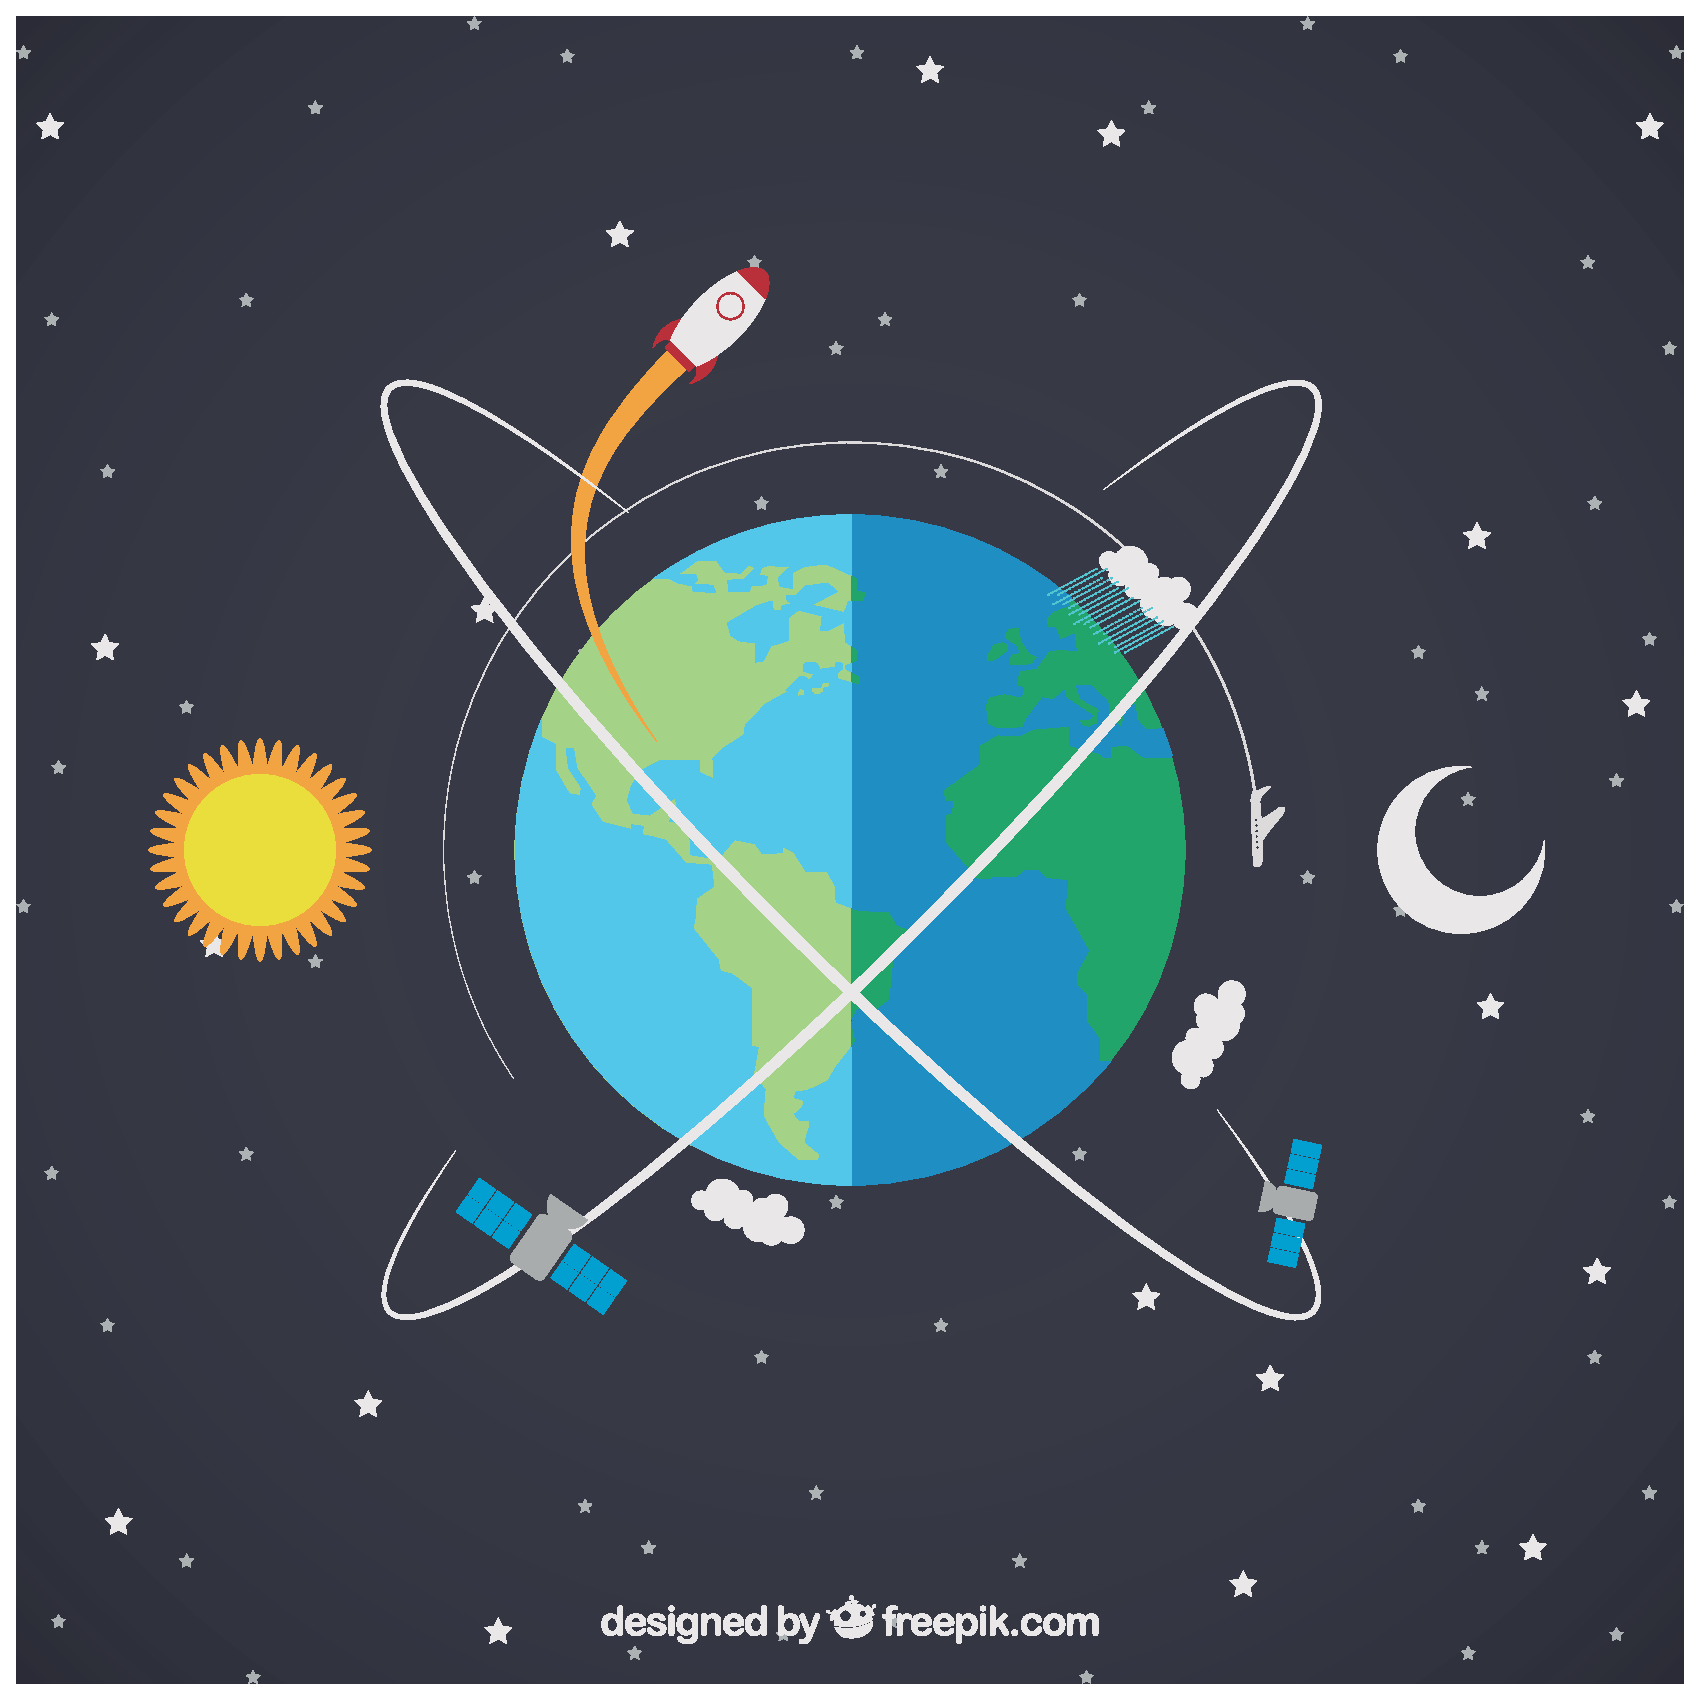
\includegraphics[width=\linewidth]{earth.eps}
}
\end{center}
\end{column}
\end{columns}
\end{example}
\end{frame}

\begin{frame}
\begin{example}
\begin{columns}
\begin{column}{0.58\linewidth}
\includegraphics[width=\linewidth]{popcorn.eps}
\end{column}
\begin{column}{0.4\linewidth}
\onslide<1->{%
Consider making popcorn. You put some oil and corn kernels in a pan and start heating.}

\vspace{2mm}
\onslide<2->{%
For the first few minutes nothing happens, then a few kernels start to pop. A little while later more and more start to pop. This goes one for a minute or so, and the popping gradually tappers off.}

\vspace{2mm}
\onslide<3->{%
Most of the popping happens in that brief, noisy moment. This demonstrates a typical pattern that is part of many phenomena.}
\end{column}
\end{columns}
\end{example}
\end{frame}

\begin{frame}[fragile]
\begin{definition}
A \textbf{normal distribution} is a perfectly symmetric, bell-shaped distribution. It is also referred to as a \textbf{normal curve} or a \textbf{bell curve}.
\begin{center}
\begin{asy}
size(320);

shade_below(0, 0.3, 0, -1.5, 1.5);
draw(normal_dist(0, 0.3, -1.5, 1.5));
draw((0,0)--(0,1.45));

xaxis();
//yaxis();

label(minipage("Mean Median Mode", 30),(.8,1.1));
draw((.8,1.25){up}..{left}(0.01,1.4),Arrow);

label("Lower 50\%", (-0.3,0.15));
label("Upper 50\%", (0.3,0.15));

draw((-1,-0.1)--(1,-0.1), Arrows);
label("Curves continues forever in both directions", (0, -0.2));

label(minipage("Curve never touches the $x$-axis", 45), (-1.2,0.15));
\end{asy}
\end{center}
\end{definition}
\end{frame}

\begin{frame}
\begin{block}{Note}
It is extremely important you master the procedures in this section. We will be using normal distributions often throughout the remainder of the course.
\end{block}\pause

\begin{block}{Equation}
The equation for the normal curve is
\begin{equation*}
y=\dfrac{e^{-\tfrac{1}{2}z^2}}{\sigma\sqrt{2\pi}}
\qquad\text{where}\qquad
z=\dfrac{x-\mu}{\sigma}
\end{equation*}
\end{block}\pause

\begin{block}{Note}
We will not be working directly from the equation in this course. 

\vspace{2mm}
The equation is only included for the rare chance you encounter technology that doesn't already have the normal distribution included.
\end{block}
\end{frame}

\begin{frame}[fragile]
\begin{definition}
The graph of any continuous probability distribution is called a \textbf{density curve} if the total area under the curve is exactly 1.
\end{definition}\pause

\begin{block}{Note}
This means there is a correspondence between the area under a density curve and probability.
\end{block}\pause

\begin{definition}
When $\mu=0$ and $\sigma=1$, the curve is called the \textbf{standard normal distribution}. The total area under its density curve is equal to 1.
\begin{center}
\begin{asy}
size(300, 75, IgnoreAspect);

draw((1,0)--(1,0.5), red);
draw((-1,0)--(-1,0.5), red);

draw(normal_dist(0, 1, -4, 4));
draw((0,0)--(0,0.5));

xaxis(Bottom(), RightTicks(NoZero, size=nan));
yaxis(Left(), LeftTicks(size=nan),ymin = 0, ymax = 0.5);

label("$\mu+\sigma$", (1, 0.45), UnFill);
label("$\mu-\sigma$", (-1, 0.45), UnFill);
\end{asy}
\end{center}
\end{definition}
\end{frame}

\begin{frame}[fragile]
\begin{definition}
The \textbf{empirical rule}, or \textbf{68-95-99.7 rule}, states approximately how much of the area is contained when stepping one, two, or three standard deviations from the mean.
\begin{overprint}
\onslide<1>
One standard deviation from the mean.
\begin{center}
\begin{asy}
size(300, 170, IgnoreAspect);

shade_between(0,1,-1,1);
draw(normal_dist(0, 1, -5, 5));
draw((0,0)--(0,0.45));

label("\Large\textbf{68\%}", (0,0.1), white);

xaxis(Bottom(), RightTicks(new real [] {-4,-3,-2,-1,0,1,2,3,4}, size=nan, ticklabel = new string(real x) { if (x == 0) return "$\mu$"; else return "$" + string(x) + "\sigma$";}));
\end{asy}
\end{center}
\onslide<2>
Two standard deviations from the mean.
\begin{center}
\begin{asy}
size(300, 170, IgnoreAspect);

shade_between(0,1,-2,2);
draw(normal_dist(0, 1, -5, 5));
draw((0,0)--(0,0.45));

label("\Large\textbf{95\%}", (0,0.1), white);

xaxis(Bottom(), RightTicks(new real [] {-4,-3,-2,-1,0,1,2,3,4}, size=nan, ticklabel = new string(real x) { if (x == 0) return "$\mu$"; else return "$" + string(x) + "\sigma$";}));
\end{asy}
\end{center}
\onslide<3>
Three standard deviations from the mean.
\begin{center}
\begin{asy}
size(300, 170, IgnoreAspect);

shade_between(0,1,-3,3);
draw(normal_dist(0, 1, -5, 5));
draw((0,0)--(0,0.45));

label("\Large\textbf{99.7\%}", (0,0.1), white);

xaxis(Bottom(), RightTicks(new real [] {-4,-3,-2,-1,0,1,2,3,4}, size=nan, ticklabel = new string(real x) { if (x == 0) return "$\mu$"; else return "$" + string(x) + "\sigma$";}));
\end{asy}
\end{center}
\onslide<4>
For each standard deviation from the mean.
\begin{center}
\begin{asy}
size(300, 170, IgnoreAspect);

shade_between(0, 1,-4, -3, white);
shade_between(0, 1,-3, -2, green);
shade_between(0, 1,-2, -1, royalblue);
shade_between(0, 1,-1,  0, orange);
shade_between(0, 1, 0,  1, fuchsia);
shade_between(0, 1, 1,  2, purple);
shade_between(0, 1, 2,  3, mediumcyan);
shade_between(0, 1, 3,  4, yellow);

draw((0,0)--(0,0.45));

real nd_func(real x, real mu, real sigma) { return 1/sqrt(2*pi*sigma*sigma)*exp((-1*(x-mu)*(x-mu))/(2*sigma*sigma)); }

void sndlabel(string s, pair pt, real offset=0.01)
{
	pair c = (pt.x, nd_func(pt.x, 0, 1) + offset);
	
	draw(pt -- c, EndArrow);
	label(s , pt, UnFill());
}

sndlabel("34\%",   (-0.5, 0.43));
sndlabel("34\%",   ( 0.5, 0.43));
sndlabel("13\%",   (-1.5, 0.25));
sndlabel("13\%",   ( 1.5, 0.25));
sndlabel("2.35\%", (-2.5, 0.15));
sndlabel("2.35\%", ( 2.5, 0.15));
sndlabel("0.1\%",  (-3.5, 0.05));
sndlabel("0.1\%",  ( 3.5, 0.05));

xaxis(Bottom(), RightTicks(new real [] {-4,-3,-2,-1,0,1,2,3,4}, size=nan, ticklabel = new string(real x) { if (x == 0) return "$\mu$"; else return "$" + string(x) + "\sigma$";}));
\end{asy}
\end{center}
\end{overprint}
\end{definition}
\end{frame}

\begin{frame}
\begin{definition}
A \textbf{z-score} is a measure of the number of standard deviations a particular data point is away from the mean. It is calculated with:
\begin{equation*}
z=\dfrac{\left(\text{data point}\right)-\left(\text{mean}\right)}{\text{standard deviation}}=\dfrac{x-\mu}{\sigma}
\end{equation*}
\end{definition}\pause

\begin{example}
On a college entrance exam, the mean was 70, and the standard deviation was 8. Rose scored a 85, what is her $z$-score?\pause

\begin{equation*}
z=\dfrac{x-\mu}{\sigma}\pause=\dfrac{85-70}{8}\pause\approx 1.875
\end{equation*}

\vspace{-4.3mm}
\end{example}\pause

\begin{example}
On the same exam, George has a $z$-score of $-1.3$. What was his score?\pause
\begin{equation*}
z=\dfrac{x-\mu}{\sigma}\pause
\quad\Rightarrow\quad
z\sigma=x-\mu\pause
\quad\Rightarrow\quad
x=z\sigma+\mu\pause = \left(-1.3\right)\left(8\right)+70=59.6
\end{equation*}

\vspace{-4.5mm}
\end{example}
\end{frame}

\begin{frame}
\begin{example}
The mean on a exam was 82, with a standard deviation of 7 points. An \textquote{A} on the exam is a 93, what is the $z$-score?\pause
\begin{equation*}
z=\dfrac{x-\mu}{\sigma}=\dfrac{93-82}{7}\approx 1.57
\end{equation*}
\end{example}\pause

\begin{note}
We know from the empirical rule that roughly 68\% of the scores fall within one standard deviation of the mean. This means that 68\% of the students scored between 75 and 89.\pause

\vspace{2mm}
Moreover, we know that roughly 95\% of the scores fall within two standard deviations of the mean. Which means that $95\%-68\%=32\%$ of the scores are more than one standard deviation from the mean, but less than two. \pause

\vspace{2mm}
Since the curve is symmetric, we know that 16\% of the students scored between 89 and 96, as well as 16\% between 68 and 75
\end{note}
\end{frame}

\begin{frame}[fragile]
\begin{definition}
An \textbf{inflection point} is where a curve changes from being concave up to concave down, or vice versa
\end{definition}\pause

\begin{note}
A normal density curve always has two inflection points, each one standard deviation from the mean.
\begin{center}
\begin{asy}
size(300, 140, IgnoreAspect);

real nd_func(real x, real mu, real sigma) { return 1/sqrt(2*pi*sigma*sigma)*exp((-1*(x-mu)*(x-mu))/(2*sigma*sigma)); }

draw(normal_dist(0, 1, -5, 5));
draw((0,0)--(0,nd_func(0,0,1)));

draw((1,0) -- (1,0.45), red);
draw((0,nd_func(1,0,1)) -- (1,nd_func(1,0,1)), red);
dot((1,nd_func(1,0,1)), red);

label("Inflection point", (1,nd_func(1,0,1)), E);

draw((-1,0) -- (-1,0.45), red);
draw((0,nd_func(-1,0,1)) -- (-1,nd_func(-1,0,1)), red);
dot((-1,nd_func(-1,0,1)), red);

label("Inflection point", (-1,nd_func(-1,0,1)), W);

label("Concave up", (2,nd_func(2,0,1)), E);
label("Concave up", (-2,nd_func(-2,0,1)), W);

label("Concave down", (0,nd_func(0,0,1)), N);

xaxis(Bottom(), RightTicks(new real [] {-4,-3,-2,-1,0,1,2,3,4}, size=nan, ticklabel = new string(real x) { if (x == 0) return "$\mu$"; else return "$" + string(x) + "\sigma$";}));
\end{asy}
\end{center}
\end{note}
\end{frame}



\begin{frame}[fragile]
\begin{example}
\begin{center}
\begin{asy}
size(300, 50, IgnoreAspect);

draw(normal_dist(0, 1, -4, 4));
shade_between(0,1,-4,0.8);
//draw((0,0)--(0,0.5));

xaxis(Bottom(), RightTicks(new real[] {0,0.8}, ticklabel=new string(real x) { if (x==0) return "0"; else return "$x$";}, size=nan));
//yaxis(Left(), LeftTicks(size=nan),ymin = 0, ymax = 0.5);
\end{asy}
\end{center}
The area of the shaded region is the probability that a $z$ score is less than or equal to $x$, $\prob{z\leq x}$.
\end{example}\pause

\begin{example}
\begin{center}
\begin{asy}
size(300, 50, IgnoreAspect);

draw(normal_dist(0, 1, -4, 4));
shade_between(0,1,-0.8,4);
//draw((0,0)--(0,0.5));

xaxis(Bottom(), RightTicks(new real[] {0,-0.8}, ticklabel=new string(real x) { if (x==0) return "0"; else return "$x$";}, size=nan));
//yaxis(Left(), LeftTicks(size=nan),ymin = 0, ymax = 0.5);
\end{asy}
\end{center}
The area of the shaded region is the probability that a $z$ score is greater than or equal to $x$, $\prob{z\geq x}$. Can also be calculated as $1 - \prob{z\leq x}$.
\end{example}
\end{frame}

\begin{frame}[fragile]
\begin{example}
\begin{center}
\begin{asy}
size(300, 50, IgnoreAspect);

draw(normal_dist(0, 1, -4, 4));
shade_between(0,1,-0.7,1.2);
//draw((0,0)--(0,0.5));

xaxis(Bottom(), RightTicks(new real[] {0,-0.7, 1.2}, ticklabel=new string(real x) { if (x==0) return "0"; else if (x < 0) return "$x_1$"; else return "$x_2$";}, size=nan));
//yaxis(Left(), LeftTicks(size=nan),ymin = 0, ymax = 0.5);
\end{asy}
\end{center}
The area of the shaded region is the probability that a $z$ score lies between $x_1$ and $x_2$, $\prob{x_1\leq z\leq x_2}$. 

\vspace{2mm}
Can also be calculated as $\prob{x\leq x_2} - \prob{z\leq x_1}$.
\end{example}\pause

\begin{note}
It is common for technology to only calculate $\prob{z\leq n}$.
\end{note}\pause

\begin{note}
It is always a very good idea to sketch a graph, shading the area you want to find. You can then determine how to find the desired area by working with cumulative areas from the left.
\end{note}
\end{frame}
\end{document}
